\section{Methods}
\label{sxn:methods}

We assume we are given several pretrained Deep Neural Networks (DNNs), as part of a similar architecture.
We would like to estimate the trends in the reported test / generalization accuracy accross a series of similar archtectures.  
and without Batch Normalization, trained on ImageNet, and widely available in the pyTorch distribution.

\paragraph{Empirical Complexity Metrics}
To do this, we will compute a variety of \emph{Complexity Metrics} based on the Product Norm of the layer weight matrics.
Note that unlike traditional ML approaches, however, we do not seek a bound on the complexity (i.e. test error), 
nor are we trying to evaluating a single model with differing hyperparmeters.  We wish to examine different models a 
common architecture series. And, also, compare different architectures themselves.  

Let us write the Energy Landscape (or optimization function) for a typical DNN with $L$ layers as
\begin{equation}
E_{DNN}=h_{L}(\mathbf{W}_{L}\times h_{L-1}(\mathbf{W}_{L-1}\times h_{L-2}(\cdots)+\mathbf{b}_{L-1})+\mathbf{b}_{L})  .
\label{eqn:dnn_energy}
\end{equation}

with activation functions $h_{l}(\cdot)$,  weight matrices $\mathbf{W}_{l}$, and the biases $\mathbf{b}_{l}$.

The model has been (or will be) trained on (unspecified) labeled data $\{d_{i},y_{i}\}\in\mathcal{D}$, 
using Backprop, by minimizing some (also unspecified) loss function $\mathcal{L}()$.  Moreover, we expect that most well trained,. production quality models will employ 1 or more forms of on regularization, such as Batch Normalization, Dropout, etc, and will also contain additional structure such as Skip Connections etc. Here, we ignore these details, and focus only on the weight matrices. 

Each layer contains by one or more layer 2D weight matrices $\mathbf{W}_{L}$, and/or the 2D feature maps $\mathbf{W}_{i,L}$ extracted from 2D Convolutional layers.  (For notational convenience, we may drop the $i$ and/or $i,l$ subscripts below.) We assume the layer weight matrices are statistically independent, allowing us to estimate the Complexity $\mathcal{C}$, or test accuracy, with a standard Product Norm, which resembles a data dependent VC complexity

\begin{equation}
\mathcal{C}\sim\Vert\mathbf{W}_{1}\Vert\times\Vert\mathbf{W}_{2}\Vert\cdots\Vert\mathbf{W}_{L}\Vert ,
\end{equation}
where $\mathbf{W}$ is an $(N\times M)$ weight matrix, with $N\ge M$, and 
 $\Vert\mathbf{W}\Vert$ is a matrix norm.   We will actually compute the log Complexity, which takes the form 
of an Average Log Norm:
\begin{eqnarray*}
\log\mathcal{C} &\sim& \log\Vert\mathbf{W}_{1}\Vert+\log\Vert\mathbf{W}_{2}\Vert\cdots\log\Vert\mathbf{W}_{L}\Vert
\end{eqnarray*}

Here, we will consider the following Norms:

\begin{itemize}
 \item Frobenius Norm: $\Vert\mathbf{W}\Vert^{2}_{F}=\Vert\mathbf{W}\Vert^{2}_{2}=\sum_{i,j}w^{2}_{i,j}$
 \item Spectral Norm:  $\Vert\mathbf{W}\Vert_{\infty}=\lambda_{max}$
 \item $\alpha-$Norm (or Shatten Norm) $\Vert\mathbf{X}\Vert^{\alpha}_{\alpha}=\sum_{i=1}^{M}\lambda^{\alpha}$,
\end{itemize}

where $\lambda_{i}$ is the $i-th$ eigenvalue of the \emph{Empirical Correlation Matrix}

\begin{equation}
\mathbf{X}=\mathbf{W}^{T}\mathbf{W}
\end{equation}

and $\lambda_{max}$ is the maximum eigenvalue. These eigenvalues are the square of the singular values $\sigma_{i}$ of $\mathbf{W}$ :  $\lambda_{i}=\sigma^{2}_{i}$.

The exponent $\alpha$ is the power law exponent that arises in our \emph{Theory of Heavy Tailed Self Regularization}, and is the determined by fitting the Empirical Spectral Density (ESD) of $\mathbf{X}$--i.e. a histogram of the eigenvalues--$\rho(\lambda)$ to a truncated power law

\begin{equation}
\rho(\lambda)\sim\lambda^{\alpha},\;\;\lambda\le\lambda_{max}
\end{equation}

We will also consider an approximate capacity metric, $\hat{\alpha}$, shown previously to correlate well with the trends in reported test accuracies of pretrained DNNs \cite{MM}

\begin{itemize}
 \item $\hat{\alpha}=\alpha\log\lambda_{max}\approx\log\Vert\mathbf{X}\Vert^{\alpha}_{\alpha}$
\end{itemize}

which approximates the log $\alpha-$Norm for both Very Heavy Tailed weight matrices ($\alpha < 2)$  and reasoably well for finite size, Moderately Heavy Tailed ones $\alpha\in[2,5]$.  


\paragraph{Spectral Analysis of Convolutional 2D Layers}
While we can easily analyze Linear layers, there is some ambiguity in performing spectral analysis on Convolutional 2D (Conv2D) layers.  A Conv2D layer is a 4-index tensor of dimension $(w,h,in\_ch,out\_ch)$, specified by an $(w\times h)$ filter (or kernel), and $in\_ch,out\_ch$ input and output channels, respectively.  Typically, the $w=h=k$,  giving $(k\times k)$ tensor slices, or \emph{pre-Activation Maps} $\mathbf{W}_{i,L}$ of dimension $(in\_ch\times out\_ch)$ each.  Usually $in\_ch\le out\_ch$.

There are at least 3 different approaches to computing the Singular Values Decomposition(s) (SVD) of an Conv2D layer
\begin{enumerate}
\item run SVD on each of the pre-Activation Maps $\mathbf{W}_{i,L}$, yielding $(k\times k)$ sets of $M$ singular values. 
\item stack the feature maps into a single rectangular matrix of, say, dimension $((k\times k\times out\_ch)\times in\_ch)$, yielding $in\_ch$ singular values
\item Compute the 2D Fourier Transform (FFT) for each of the $(in\_ch, out\_ch)$ pairs, and run SVD on the resulting Fourier coeffients\cite{Long2019}.  This leads to $\sim(k\times in\_ch\times out\_ch)$ non-zero singular values.
\end{enumerate}

Each method has tradeoffs.  While, in principle, 3. is mathematically sound, it is computationally expensive. 
For this study, because we are computing tens of thousands of calculations, we select $1.$, which is 
numerically the fastest and easiest to reproduce.\footnote{We will provide a Google Colab notebook where all results can be reproduced, with the option to redo the calculations with option 3 for the SVD of the Conv2D.}

To verify that our approach is meaningful, we need to see the ESD is neither due to a random matrix, nor due to unsually large matrix elements, but, in fact, captures correlations learned from the data.  We examine typical Conv2D layer for the pretained AlexNet model (distributed with pyTorch).  Figure \ref{fig:alexnet1} displays the ESD for the first slice (or matrix $\mathbf{W}$) of the third Conv2D layer, extracted from a 4-index Tensor of shape $(384, 192, 3, 3)$.  The red line displays the best fit to a random matrix, using the Marchenko pastur theory\cite{MM}.  We can see the random matrix model does not describe the ESD very well. For comparison, Figure \ref{fig:alexnet2} shows the ESD of the same matrix, randomly shuffled; here looks similar to the red line plot of the orginal ESD.  In fact, the empircal ESD is better modeled with a truncated power law distribtion.

Although the ESD is \emph{Heavy Tailed}, this does not imply that the orginal matrix $\mathbf{W}$ is itself heavy tailed--
only the correlation matrix $\mathbf{X}$ is. If $\mathbf{W}$ was, 
then it would contain 1 or more unusually large matrix elements, and they would dominate the ESD.  
Of course the randomized $\mathbf{W}$ would also be heavy tailed, but its ESD neither resembles the original
nor is it heavy tailed.  So we can rule out $\mathbf{W}$ being heavy tailed.

\begin{figure}[H]
   \centering
   \subfigure[Actual ESD]{
     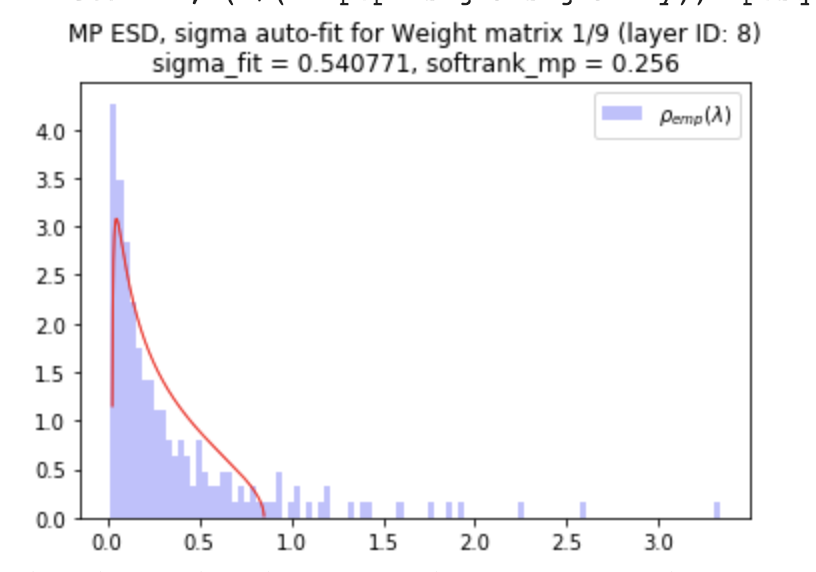
\includegraphics[scale=0.5]{img/alexnet1.png} 
     \label{fig:alexnet1}
   }
   \subfigure[ESD of randomly shuffled matrix]{
      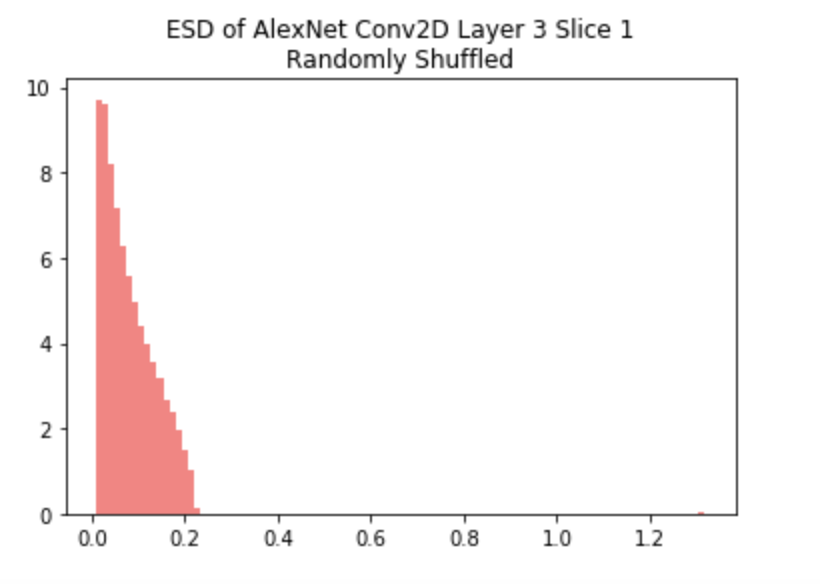
\includegraphics[scale=0.5]{img/alexnet2.png}
      \label{fig:alexnet2}
   }
   \caption{ESD of AlexNet Conv2D pre-Activation map for Layer 3 Slice 1, actual and randomized}
   \label{fig:alexnet}
\end{figure}


These plots tell us that the pre-activation maps of the Conv2D contains significant correlations learned from the data.  
By modeling the ESD with a power law distribution $\lambda^{\alpha}$, we can characterize the amount of correlation learned;
the smaller the exponent $\alpha$, the more correlation in the weight matrix. 

\paragraph{Normalization of Empirical Matrices}.  
The normalization does not affect the Power Law fits because the Heavy Tailed exponent $\alpha$ is scale-invariant.
As are metrics like the Stable Rank and our MP Soft Rank. In this study, however, all of the metrics strongly depend 
on the scale of the weight matrix.
Formally, to apply RMT, we would usually define Correlation Matrix with $\dfrac{1}{N}$ normalization,
and assume that either the variance of $\mathbf{X}$ is unity, $\sigma^{2}=1$, or is known.
\footnote{And for formal proofs of the Heavy Tailed results, we need a different normalization,$\dfrac{1}{N^{1-\alpha}}$}
But for these empirical studies, the pretrained DNNs are typically initialized with random weight matrices $\mathbf{W}_{0}$ ,
with the variance already normalized to $\sqrt{\frac{1}{N}}$, or some variant of this such as Glorot (or Xavier) Normalization\cite{GloRot},
or as $\sqrt{\frac{2}{N*k^2}}$ for Convolutional 2D Layers. 
We do not normalize (or renormalize) the Empirical Correlation Matrices, and use them as-is,
except that we rescale the Conv2D pre-Activation Maps $\mathbf{W}_{i,L}$ by $\frac{k}{\sqrt{2}}$ so that they
are on the same scale as the Linear layers.


Note that in some pretrained models, like the pyTorch VGG models, the Linear weight matrices appear to have been 
initialized with variance $\sigma\sim0.01$.  We do not attempt to correct for this, and, instead, simply try to treat all
models the same.  

COMMENT ON HOW LOG NORM first and last layers behave, maybe somewhere else

COMMENT ON HOW LOG PORM  for GPT includes unusually high alpha, not meaningful other than to show the trend.

\paragraph{The WeightWatcher Tool}


\paragraph{Organization of this paper}

We want to study the effective of Product Norm Metrics in describing trends in the
generalization accuracyof real-word, production quality, pretrained Deep Neural Networks.
In Section \ref{sxn:cv}, we study three well known, and widely available DNN CV architectures:
the VGG series, the ResNet series, and the DenseNet series of models.  We lay out the
basic methodology we use to evaluate the different metrics against the reported test accuracies. 
We also introduce the notion of Correlation Flow, compare the three pretrained architectures in detail.  
In Section  \ref{sxn:nlp}, we then look at several variations of a popular NLP DNN architecture,
the OpenAI GPT and GPT2 models.  We discuss when and how the different metrics apply more generally.
Finally, in Section \ref{sxn:all}, we examine over 100 pretraind DNN CV models, and show
how well each metric is correlated with the reported test accuracies across different models
in an architeture series.  
----








